% !TEX root = ../main.tex

\section{Sequential Monte Carlo}
\label{sec:part:smc}

\subsection{Non-Markovian State-Space Models}
\label{sec:part:smc:nmssm}

\begin{figure}[t]
	\centering 
	% !TEX root = ../main.tex

\begin{tikzpicture}

\node[latent, minimum size=27pt] (x1) {$x_1$};
\node[latent, right=1.4cm of x1, minimum size=27pt] (x2) {$x_2$};
\node[right=1.4cm of x2] (x3) {{\tiny $\bullet \; \bullet \; \bullet$}};
\node[latent, right=1.4cm of x3, minimum size=27pt] (x4) {$x_{T\text{-}1}$};
\node[latent, right=1.4cm of x4, minimum size=27pt] (xT) {$x_T$};

\node[obs, below=of x1, minimum size=27pt] (y1) {$y_1$};
\node[obs, below=of x2, minimum size=27pt] (y2) {$y_2$};
%\node[obs, below=of x3] (y3) {$y_3$};
\node[obs, below=of x4, minimum size=27pt] (y4) {$y_{T\text{-}1}$};
\node[obs, below=of xT, minimum size=27pt] (yT) {$y_T$};

%\node[latent, above=of x1, xshift=-1.2cm, minimum size=27pt] (t) {$\theta$};

\edge {x1} {x2,y1} ; %
\edge {x2} {x3,y2} ; %
\edge {x3} {x4} ; %
\edge {x4} {xT,y4} ; %
\edge {xT} {yT} ; %

%\edge {t} {x1,x2};
%\edge[bend left=0] {t} {x4};
%\edge[bend left=10] {t} {xT};

\edge[bend left=30] {x1} {x4}
\edge[bend left=35] {x1} {xT}
\edge[bend left=20] {x2} {xT}

\edge[bend left=0] {x1} {y2,y4,yT}
\edge[bend left=10] {x2} {y4,yT}
\edge[bend left=0] {x4} {yT}

\end{tikzpicture}
	\caption{DAG for a non-Markovian state space model.  Note there are all also multiple dependencies
		for the nodes summarized by the dots.
		\label{fig:part:nmssm}}
\end{figure}

Although SMC can be used for an arbitrary series of targets as we will explain
in Section~\ref{sec:part:smc:arb}, we will mostly introduce it in the context of non-Markovian state-space
models (NMSSMs).  NMSSMs are probabilistic models over a set of latent variables 
$x_t \in \mathcal{X}_t, \; \forall t = 1:T$
and observed variables $y_t \in \mathcal{Y}_t, \forall t = 1:T$.  
%We can further consider the model to be parameterized by $\theta \in \Theta$ which
%we will for now presume is known.
They are similar to
the HMM introduced in~\ref{sec:bayes:paradigm:graph}, but differ by not
making the Markov assumption.  This leads to the graphical model shown in Figure~\ref{fig:part:nmssm}.
They are fully defined by an initial density $\mu (x_1)$,
a series of transition densities $f_{t} (x_t | x_{1:t-1})$, and a series of
emission densities $g_{t} (y_t | x_{1:t})$ as follows
\begin{subequations}
\label{eq:part:ssm}
\begin{align}
x_1 &\sim \mu(x_1), \\
x_t | x_{1:t - 1} &\sim f_{t}(x_t | x_{1:t - 1}), \\
y_t | x_{1:t} &\sim g_{t}(y_t | x_{1:t}).
\end{align}
\end{subequations}
which gives a joint density of
\begin{align}
\label{eq:part:jointdistribution}
p(x_{1:T}, y_{1:T}) = \mu(x_1) \prod_{t = 2}^T f_{t}(x_t | x_{1:t - 1}) \prod_{t = 1}^T g_{t}(y_t | x_{1:t})
\end{align}
and the standard relationship that this is proportional to the posterior
$p(x_{1:T} | y_{1:T})$.  Note the
key self-similarity relationship: the intermediate posterior of the first $t$ latent variables
given the first $t$ observations is
\begin{align*}
p(x_{1:t} | y_{1:t}) \propto \mu(x_1) \prod_{\tau = 2}^t f_{\tau}(x_{\tau} | x_{1:\tau - 1}) \prod_{\tau = 1}^t g_{\tau}(y_{\tau} | x_{1:\tau}).
\end{align*}
Perhaps surprisingly, this framework can be almost completely general if the $x_t$ and $y_t$
are allowed to take on arbitrary form.  For example, if we set $T=1$ then $x_1=\theta$ are our variables,
$y_1 = \mathcal{D}$ is our data, $\mu(x_1) = p(\theta)$ is our prior, and $g_1(y_1|x_1)=p(\mathcal{D}|\theta)$
is our likelihood.  More generally, the initial density and transition densities form terms in the
prior, while the emission densities are terms in the likelihood; all of which can take on arbitrary forms.
It will often be the case that each ``latent variable'' is actually a collection of different variables and
each ``observed variable'' is actually a collection of observations.
What the NSMSSM formulation allows us to do is express known structure present in the problem: 
the earlier we are able to put our observations in the observation structure, and thus express their conditional
independence from more of the latent variables, the more will be able to exploit this structure.

There are two common tasks that one wishes to carry out for NMSSMs: \emph{filtering} and
\emph{smoothing}.  Smoothing corresponds to the standard Bayesian inference task where we
want to infer about the latent variables conditioned on all the observations.  In filtering
we care about the posterior given the observations
so far $p(x_t | y_{1:t})$.  Filtering is typically done in tasks such as tracking and signal
processing where the inference is being done online and the main task is forward prediction.
In other words, we do not know all the $y_{1:T}$ upfront but have a series of inference problems
where we wish to predict $y_{t+1},y_{t+2},\dots$ given the observations so far $y_{1:t}$.  Our
focus will be on smoothing, but we note that this is equivalent to the filtering distribution
at the last step and so most of the ideas directly transfer.

If the model is in fact Markovian with Gaussian or discrete transition distributions and Gaussian
emission distributions, then the posterior can be calculated analytically using the \emph{Rauch-Tung-Striebel}
smoother~\citep{rauch1965maximum} and \emph{forward-backward} algorithm~\citep{rabiner1986introduction} respectively.
The former corresponds to the class of Kalman filter~\citep{kalman1960new} and Kalman smoother~\citep{rauch1965maximum}
algorithms.  These are often used for Bayesian modeling of dynamics and
are a good example of where approximations are often made in Bayesian approaches in the interest of
tractability.  SMC will allow us to perform inference in similar models, amongst many others, without requiring
such assumptions to be made.  Naturally, this will come at the cost of having access to a closed-form solution.

\subsection{Sequential Importance Sampling}
\label{sec:part:smc:sis}

In Section~\ref{sec:inf:foundation:importance:unk-f} we showed that importance sampling weights
are multiplicative and thus to sample from a joint
distribution, one can first importance sample from a marginal distribution and then importance
sample from the respective conditional distribution, with the sample weight corresponding to the
product of the two individual weights.  More generally, one can carry out \emph{sequential importance
	sampling} (SIS) to carry out inference on a series of target distributions $(\pi_t(x_{1:t}))_{t = 1}^T$ of 
increasing spaces $\mathbb{X}_1,\dots,\mathbb{X}_T$ where each
$\mathbb{X}_t = \mathcal{X}_1 \times \dots \times \mathcal{X}_t$, $x_t\in\mX_t$ by first making
an importance sampling approximation for $\pi(x_1)$ and sequentially update our approximation from
$\pi_t(x_{1:t})$ to $\pi_{t+1}(x_{1:t+1})$ by doing importance sampling updates and taking the product of
the weights.  This is easiest to see in the NMSSM case using the series of targets $p(x_{1:t}|y_{1:t})$
which we can do by first approximating $p(x_1 | y_1)$ and then importance sampling each 
\[
p (x_t | x_{1:t-1}, y_{1:t})=p(x_t | x_{1:t-1}, y_t)\propto f_{t}(x_t | x_{1:t-1}) g_{t}(y_t | x_{1:t})
\]
noting that $x_t$ is independent of $y_{1:t-1}$ given $x_{1:t-1}$.  
Presuming a set of proposals 
$q_1(x_1), q_t(x_t | x_{1:t-1})$, we will calculate importance weights as follows
\begin{subequations}
	\label{eq:part:sis-weights}
\begin{align}
w_1 (x_1) &= \frac{\mu (x_1)g_{t}(y_1 | x_1)}{q_1(x_1)} \\
w_t (x_{1:t}) &= w_{t-1} (x_{1:t-1}) \frac{g_{t}(y_t|x_{1:t}) f_{t}(x_t | x_{1:t-1})}{q_t(x_t|x_{1:t-1})}.
\end{align}
\end{subequations}
Once completed this will produce a set of weighted sample $\{\hat{x}_{1:T},w_T(\hat{x}_{1:T})\}$ for 
$p(x_{1:T} | y_{1:T})$.  A summary of the SIS process is given in Algorithm~\ref{alg:part:sis}.

\begin{algorithm}[tb]
	\caption{Sequential Importance Sampling}
	\label{alg:part:sis}
	\begin{spacing}{1.2}
		\begin{algorithmic}[1]
			\renewcommand{\algorithmicrequire}{\textbf{Inputs:}}
			\renewcommand{\algorithmicensure}{\textbf{Outputs:}}			 
			\Require model $p(x_{1:T},y_{1:T})$, data $y_{1:T}$, proposals $q_1,\dots,q_T$, number of samples $N$
			\Ensure weighted samples $\left\{x_{1:T}^i,w_T^i\right\}_{i=1}^N$
			\For{$i=1,\dots,N$}	
			\State $x_1^i \sim q_1(x_1)$
			\State $w_1^i = \frac{g_1(y_1|x_1^i) \mu(x_1^i)}{q_1(x_1^i)}$
			\For{$t = 2$ {\bfseries to} $T$}
			\State $x_t^i \sim q_t(x_t | x_{1:t-1}^i)$ 
			\State Set $x_{1:t}^i = (x_{1:t-1}^{i},x_t^i)$
			\State $w_t^i = w_{t-1}^i \frac{g_t(y_t|x_{1:t}^i) f_t(x_t^i | x_{1:t-1}^{i})}{q_t(x_t^i|x_{1:t-1}^{i})}$
			\EndFor
			\EndFor
		\end{algorithmic}
	\end{spacing}
\end{algorithm}

Because SIS produces a pure importance sampling estimate, it will share all the desirable properties
of importance sampling introduced in Section~\ref{sec:inf:foundation:importance}, including the
ability to use self-normalization.  In fact, it is just
a particular case of importance sampling because could have produced the same samples and weights
by sampling $x_{1:T} \sim q_1(x_1) \prod_{t=2}^{T} q_t (x_t | x_{1:t-1})$ and then calculating the
corresponding importance weight $w_T(x_{1:T})$ in one go. As such, 
SIS is on its own not very useful.  Its utility is realized when it is combined with resampling as we describe next.

\subsection{SMC for Non-Markovian State Space Models}
\label{sec:part:smc:smc-nmssm}

Sequential Monte Carlo (SMC)~\citep{gordon1993novel,doucet2001sequential,doucet2009tutorial} , or particle filtering 
as it is sometimes known,\footnote{We avoid the name
	particle filtering as it often implies that one is only interested in the filtering distribution, whereas
	most of the tasks we are interested in will target the smoothing distribution.} 
is a powerful and general purpose inference algorithm that has been successfully
applied to a wide range of fields such as signal processing~\citep{candy2016bayesian}, econometrics~\citep{creal2012survey}, 
and probabilistic programming~\citep{wood2014new}.  SMC builds on SIS by interleaving the sampling
with resampling steps, the latter
of which was introduced in Section~\ref{sec:inf:foundation:resampling}.
The key idea is to exploit the structure of a model by breaking down the overall 
inference problem into a series of target distributions which get incrementally closer to the 
distribution of interest.  Transitioning from one intermediary distribution to the next typically
forms a far simpler inference problem that directly approximating the original target.  The critical difference
to SIS is that
the information gained from approximating these intermediary distributions is exploited by
reallocating resources to areas likely to have high posterior mass in the final target distribution
through resampling.  The simplest, but most common form of SMC, which simply interleaves
\emph{propagating} samples from one target to the next and resampling the particle system, is sometimes known
as \emph{sequential importance resampling} and will be our main focus.
A characterization of the method is shown in Figure~\ref{fig:part:smc_explan}.  

\begin{figure}[t]
	\centering 
	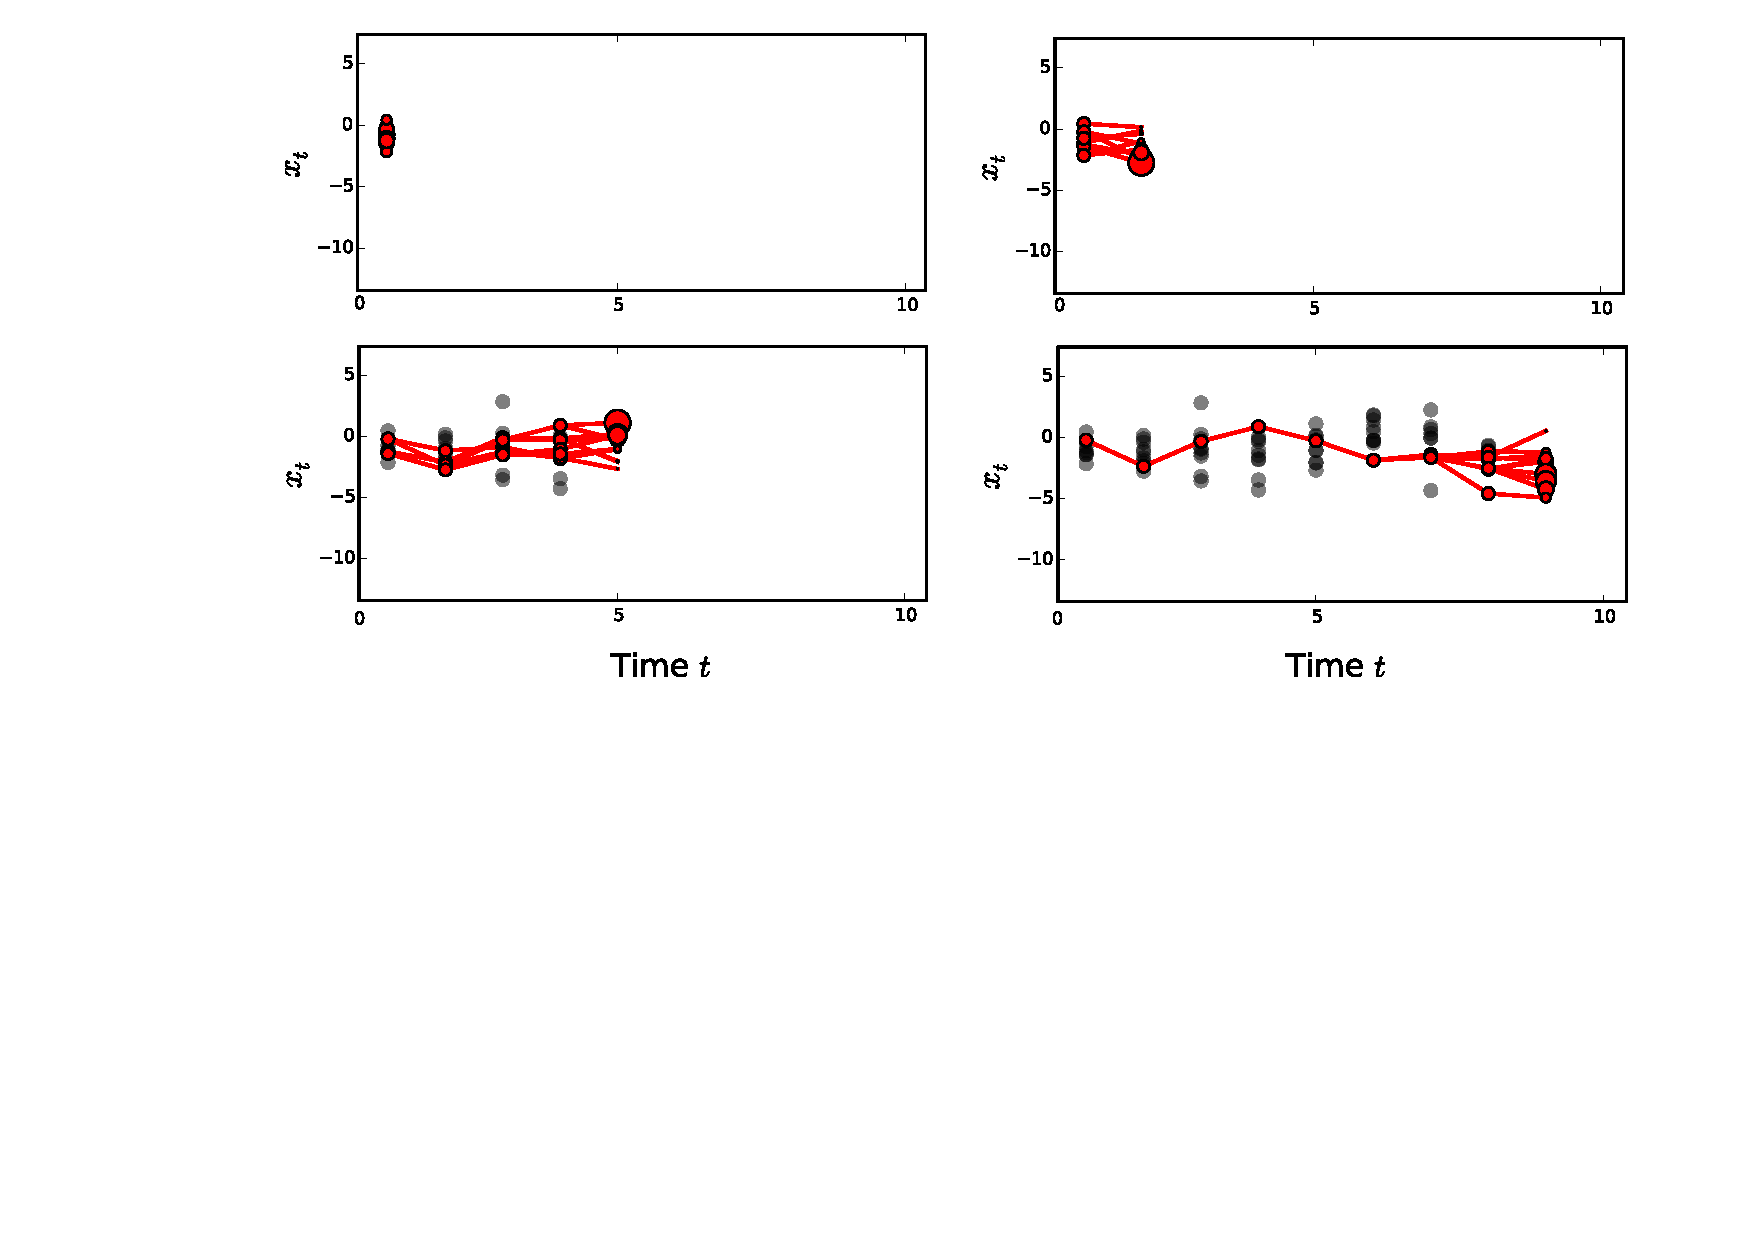
\includegraphics[width=\textwidth]{part/figures/smc_explan}
	\caption{Characterization of the SMC method for a state space model.  At the first time step (top left) 
		we perform importance sampling to approximate $p(x_1 | y_1)$ in the normal way, giving a particle system, or population
		of weighted samples $\{x_1^i,w_1^i\}_{i=1}^N$.  Here each sample is shown by a red blob whose size reflects the weight
		of the particle.  The set of particles are then resampled to produce an unweighted set of particles approximating
		$p(x_1 | y_1)$.  For each of these samples, importance sampling is then used again to produce samples for $x_2$
		by sampling from $q_2 (x_2 | x_1)$ and applying a new importance weight (top right).  Note that, unlike for SIS,
		the importance weights are not propagated from one time step to the next.
		We now again have a weight particle set $\{x_{1:2}^i,w_2^i\}_{i=1}^N$, for which we again perform a resampling
		step to produce an unweighted set of particles.  The process continues in the same way, eventually returning the
		final set of samples $\{x_{1:T}^i,\nw_T^i\}_{i=1}^N$, where we have self-normalized the final weights of each trajectory
		(note that each $\nw_T^i$ applies to the full trajectory $x_{1:T}^i$).  
		Over time, many of the generated samples are
		discarded by the system (shown in gray) during the resampling step.  A consequence of this, which can be seen
		in the bottom right, is that
		many time steps, then our particle set become \emph{degenerate}.  Here we have multiple distinct samples for $x_9$, but
		all our samples share the same \emph{ancestors} for $t=1:6$, i.e. each $x_t^i$ in our final sample set is
		the same for $t\le6$.  We will return to discuss this further in Section~\ref{sec:part:pmcmc:path-deg}.
		\label{fig:part:smc_explan}}
\end{figure}

To see the intuition of why resampling provides the desired resource reallocation, consider what happens 
to the relative weights of different particles in a population if they are propagated through the SIS algorithm at the
same time.  It is easy to see that these weights will quickly diverge, typically exponentially quickly
 (see Section~\ref{sec:inf:foundation:curse}), and our effective sample size 
(see Section~\ref{sec:inf:foundation:ess}) will rapidly diminish.  It is now rather pointless to continue to
propagate the samples with negligible weight through the system as the chance these will have a significant
weight by the end is very low.  We therefore desire a principled way of ``killing off'' these
low weight particles and replacing them with higher weight ones.  As we showed in Section~\ref{sec:inf:foundation:resampling},
resampling gives us a method for generating unweighted samples from a population of weighted samples.
Though resampling itself only duplicates existing particles, rather
than producing new ones, if the duplicate samples are extended independently at the next iteration, this
produces distinct samples (albeit heavily correlated ones).  In other words if we have two samples
$x_{1:t}^1$ and $x_{1:t}^2$ such that $w_t^2/w_t^1 \approx 0$ then it is more beneficial for us to generate both
samples at the next stage using $x_{t+1}^i \sim p(x_{t+1} | x_{1:t}^1, y_{1:t})$ for $i=1,2$, than to use
$x_{1:t}^2$ to sample $x_{t+1}^2$.  This will not improve our representation of $x_{1:t}$, but it will, in
general, give a better representation of the marginal distribution of $x_{t+1}$ and thus the joint distribution
$x_{1:t+1}$.   
%Note that any of the resampling schemes introduced in Section~\ref{sec:inf:foundation:resampling}
%will give rise to valid SMC schemes and so one should, from a practical perspective, generally
%use systematic resampling.

To introduce the \smc method more formally, we consider approximating a sequence of target distributions
in same way as for SIS: in our NMSSM
 case $p(x_{1:t}|y_{1:t}) = p(y_{1:t})^{-1} p(x_{1:t},y_{1:t}), ~t=1,\ldots,T$. 
At each time step $t$ we 
%assume we have access to 
generate a particle system
$\{x_{1:t}^i,w_{t}^i\}_{i=1}^N$ which provides a weighted approximation  to $p(x_{1:t}|y_{1:t})$. Given such a 
weighted particle system, we convert this to an unweighted particle system by resampling as explained
in Section~\ref{sec:inf:foundation:resampling}.  Any of the introduced resampling schemes can be 
used~\citep[Section 4.1]{andrieu2010particle}
and so in general one should use systematic resampling.
When we later introduce PMCMC methods, it will
be useful to think about resampling in terms of propagating particles each particle by drawing an 
ancestor variable $a_{t-1}^i$ (as per~\eqref{eq:inf:resampling}) and then using this to propose the new
variable for that particle, i.e. $x_t^i \sim q_t(x_t | x_{1:t-1}^{a_{t-1}^i})$.  The particle system is then
re-weighted as
\begin{align}
\label{eq:part:smcweights}
w_t^i = \frac{g_t(y_t|x_{1:t}^i) f_t(x_t^i | x_{1:t-1}^{a_{t-1}^i})}{q_t(x_t^i|x_{1:t-1}^{a_{t-1}^i})},
\end{align}
where $x_{1:t}^i = (x_{1:t-1}^{a_{t-1}^i},x_t^i)$.   Note that after resampling,
all the particles have the same weight and therefore, unlike for SIS, the weights at the previous step
do not feature in the weights at the current time step.
This results in a new particle system $\{x_{1:t}^i,w_t^i\}_{i=1}^N$ that approximates $p(x_{1:t}|y_{1:t})$
and the algorithm continues in a self-similar manner up to time $T$.
The overall process is detailed in Algorithm~\ref{alg:part:smc}.  Once run, we can use our final, self-normalized,
particle set $\{x_{1:T}^i,\nw_T^i\}_{i=1}^N$ as a Monte Carlo estimator in the same manner as self-normalized
importance sampling:
\begin{align}
\label{eq:part:smc-est}
\E_{\pi (x_{1:T})} \left[f(x_{1:T})\right] \approx \frac{1}{N} \sum_{i=1}^{N} \nw_T^i f(x_{1:T}^i).
\end{align}

\begin{algorithm}[tb]
	\caption{Sequential Monte Carlo \hfill {\small (all for $i=1,\ldots,N$)}}
	\label{alg:part:smc}
	\begin{spacing}{1.2}
		\begin{algorithmic}[1]
			\renewcommand{\algorithmicrequire}{\textbf{Inputs:}}
			\renewcommand{\algorithmicensure}{\textbf{Outputs:}}				 
			\Require  data $y_{1:T}$, number of particles $N$, proposals $q_t$
			\State $x_1^i \sim q_1(x_1)$
			\State $w_1^i = \frac{g_1(y_1|x_1^i) \mu(x_1^i)}{q_1(x_1^i)}$
			\For{$t = 2$ {\bfseries to} $T$}
			\State $a_{t-1}^i \sim \Discrete\left(\left\{\nw_{t-1}^{\ell}\right\}_{\ell=1}^N\right)$% \tom{We can maybe more general that categorical here?}
			\State $x_t^i \sim q_t(x_t | x_{1:t-1}^{a_{t-1}^i})$ 
			\State Set $x_{1:t}^i = (x_{1:t-1}^{a_{t-1}^i},x_t^i)$
			\State $w_t^i = \frac{g_t(y_t|x_{1:t}^i) f_t(x_t^i | x_{1:t-1}^{a_{t-1}^i})}{q_t(x_t^i|x_{1:t-1}^{a_{t-1}^i})}$
			\EndFor
		\end{algorithmic}
	\end{spacing}
\end{algorithm}

Many intuitions from importance sampling transfer over to SMC.  For example, we can construct our posterior
estimate and calculate expectations in the same way, while we can also use the effective sample size as
a metric of performance (remembering to coalesce identical samples). 
One of the most importance features that translates is that SMC produces the
unbiased estimate for the marginal likelihood $p(y_{1:T})$
\begin{align}
\label{eq:part:ML}
\hat Z = \prod_{t=1}^T \frac{1}{N} \sum_{i=1}^N w_{t}^{i}.
\end{align}
as first shown by~\cite{del2004feynman}.  Although this original
proof requires advanced techniques we will not touch on here, we will later show that this results can also be shown
as a consequence of the proof of correctness for the particle independent Metropolis-Hastings method
given in Section~\ref{sec:part:pmcmc:pimh}.  Note that although the marginal likelihood estimate is
unbiased, the estimator for an general expectation given by~\eqref{eq:part:smc-est} is biased in the same
way as the self-normalized importance sampling estimator given in~\eqref{eq:inf:snis} is.  Nonetheless, producing unbiased
estimates of the marginal likelihood has numerous significant advantages.  

Firstly, it means that one can combine
results from difference SMC runs and still have a consistent estimator for the target and a both unbiased and
consistent estimate for the marginal likelihood.
The is particularly important because the number of particles $N$, is typically restricted by the availability of memory
and we often want to run more than one \emph{SMC sweep} (i.e. single run of SMC).
To combine our estimates, one simply weights each sample by the marginal likelihood of its sweep times
its local, self-normalized, weight $\nw_T^i$, giving the estimator
\begin{align}
\label{eq:part:ind-smc}
\E_{\pi (x_{1:T})} \left[f(x_{1:T})\right] \approx \frac{1}{RN} \sum_{r=1}^{R}\sum_{i=1}^{N} \hat{Z}[r] \nw_T^i[r] f(x_{1:T}^i[r])
\end{align}
where the notation $[r]$ is used to indicates samples from sweep $r$.
 The ability to do this is known as \emph{proper weighting}~\citep{andersson2015nested} and we can justify it by
thinking in terms of using a proposal that first samples a full particle set, giving importance weight $\hat Z$, and then sampling a particle
from this set, giving importance weight $\nw_T^i$.  The product of these separate weights thus gives the weight of
each sample.  

Secondly, the unbiased marginal likelihood estimate means that we can \emph{nest} SMC within other 
methods as a unbiased estimate of the likelihood.
Methods that make use of such unbiased likelihood estimates are known as pseudo-marginal
methods~\citep{andrieu2009pseudo} and will be discussed in Chapter~\ref{chp:nest}
Some PMCMC methods we introduce in Section~\ref{sec:part:pmcmc} can also be interpreted as pseudo-marginal methods.
%
%The sequential nature of SMC and the resampling step are crucial in making SMC scalable to large $T$.
%The former makes it easier to design efficient proposal distributions as each step need only target 
%the next set of variables $x_t \in \mathcal{X}_t$. 
%The resampling step then allows the algorithm to focus on promising particles in light of new 
%observations, avoiding the exponential divergence between the weights of different samples that 
%occurs for importance sampling as $T$ increases.
%This can be demonstrated both empirically and theoretically \citep[Chapter 9]{del2004feynman}.

\subsection{Sequential Monte Carlo for an Arbitrary Series of Targets}
\label{sec:part:smc:arb}

In its most general form, we can use SMC to target an arbitrary
series of unnormalized target distributions $\left\{\gamma_t (x_{1:t})\right\}_{t=1:T}, \; 
\gamma_t (x_{1:t}) = Z_t \pi_t (x_{1:t})$, each defined on a space
$\mathbb{X}_t$ with strictly increasing dimension\footnote{This restriction
	can be relaxed by using the SMC samplers approach of \citet{del2006sequential}.}
$\mathrm{dim}(\mathbb{X}_{t-1})<\mathrm{dim}(\mathbb{X}_{t})$.
Here $Z_t := \int \gamma_t(x_{1:t}) dx_{1:t}$ is the normalization constant and $\pi_t (x_{1:t})$
the corresponding normalized target.  
The only difference that needs to be made from the NMSSM case is in how the weights
are calculated, with them now given by
\begin{subequations}
\label{eq:part:smc-arb-weights}
\begin{align}
w_1^k &= \frac{\gamma_1(x_1^k)}{q_1(x_1^k)} \\
w_t^k &= \frac{\gamma_t({x}_{1:t}^k)}{\gamma_{t - 1}({x}_{1:t - 1}^{a_{t - 1}^k}) q_t(x_t^i|x_{1:t-1}^{a_{t-1}^i})}.
\end{align}
\end{subequations}
It can be easily seen that the NMSSM weights are a particular case of this, by
plugging in $\gamma_t(x_{1:t}) = p(x_{1:t},y_{1:t})$ into the above expression.  

For inference, then our posterior is the
last target, $\pi_T (x_{1:T})$, with corresponding marginal likelihood $Z_T$.  Using this
more general SMC formulation, we thus see that any series of targets will lead
to a valid inference provided that the final target is the desired posterior and that none
of our intermediate targets place zero probability mass on events that have non-zero
probability mass under the corresponding marginals of the final target 
\begin{align}
\label{eq:part:opt-target}
\tilde{\pi}_t (x_{1:t}) = \int \pi_T (x_{1:T}) dx_{t+1:T}
\end{align}
$\ne \pi_t (x_{1:t})$ in general.  In fact, the series of targets given
for the NMSSM case are actually suboptimal and used because of the fact that
$p(x_{1:t},y_{1:t})$ can, in general, be calculated exactly.  It is a well known result
(see, for example, the appendices of~\cite{le2017auto}) that the optimal series
of proposals (complications with computability and proposals aside) is actually 
the marginals $\tilde{\pi}_t (x_{1:t})=p(x_{1:t} | y_{1:T})$ for
the NMSSM case.  To see this, note that at the $t^{\mathrm{th}}$ step, we are generating 
the samples for $x_{t}$ and so if each of targets is the marginal of the final distribution
$p(x_{1:t} | y_{1:T})$, then the marginal probability of the already sampled variables does not change from
one step to the next.  Conversely, $\pi_t (x_{1:t}) \neq \int \pi_{t+1} (x_{1:t+1}) dx_{t+1}$
in general and so if a different series of targets are used,
e.g. $p(x_{1:t}|y_{1:t})$, then the marginal probability of the already sampled
variables changes from one iteration to the next, reducing the efficient of the inference.
To give an example of this, consider
the case where $x_{1}$ include global parameters that effect each emission
distribution, for example it could contain the variance for Gaussian
likelihood terms.  In our NMSSM case we can never regenerate samples for $x_1$ after
the first step and so it is clearly better at the first step to target $p(x_1 | y_{1:T})$ than $p(x_1|y_1)$,
i.e. to condition on all the data rather than the first datapoint. Unfortunately, calculating
$p(x_1 | y_{1:T})$ itself generally requires a marginalization that is as difficult, or potentially
even more difficult, than the inference itself.  Hence the series of targets we introduced in
the NMSSM formulation are those that are usually used in practice.  However, we note that there are some
innovative methods for partially alleviating this problem, such as block sampling~\citep{doucet2006efficient} methods,
which use a combination of lookahead and \emph{auxiliary weighting} schemes~\citep{cappe2007overview}.
Specifically, they resample using adjusted weights that convey how good the sample is likely
to be a few time steps further down the line.  The bias this would induce is corrected for
by assigning non-even weights to the resampled particles.

Another upshot of the ability to use an arbitrary series of targets is that we can use SMC in scenarios that do not
permit a conventional breakdown of the target distribution, but where we 
can provide guiding distributions to that which we care about.  One possible case is when our prior distribution
is a generative model that can be evaluated on the target dataset at point in generative process.
For example, in~\cite{janz2016probstruct}, we considered the example of doing inference
on the structure of a GP kernel.  Here we can define a generative model that produces
increasingly complex kernels, such that all the intermediary kernels in this generation process are themselves
valid kernels that can thus be evaluated.  Here we can think of expanding our kernel at each time step of 
the SMC inference and our targets as being the posterior on kernel structure for the GP, subject to increasingly
lax restrictions on the kernel complexity.\footnote{Technically in this work actually uses population
	Monte Carlo~\cite{cappe2004population} which is based on using a series of static targets.  The
	intuition, however, predominantly transfers and SMC could have been used instead.}  
Another example is provided by~\cite{lakshminarayanan2013top},
who use SMC for Bayesian learning of decision trees.  Here they use the self-similarity of trees, starting
with a basic stump and then adding a new split at each time step.
For both these problems, SMC has been used
to exploit the fact that the overall problem can be broken down into a series of increasingly difficult
problems, namely those with an increasingly large prior, to guide towards good solutions for the final problem.

\subsection{Practical Considerations}
\label{sec:part:smc:prat}

\subsubsection{Use as Many Particles as Possible}
\label{sec:part:smc:prat:part}

The most important practical consideration for SMC is to
\emph{use as many particles as possible}.  Although, as we showed in~\ref{sec:part:smc:nmssm},
one can run multiple, say $R$, SMC sweeps with $N$ particles each and then combine them using their marginal likelihood estimates, this
is almost exclusively a higher variance (and more skew) estimator than carrying out a single SMC sweep
with $RN$ particles, often many orders of magnitude so.  It is easy to see why a single sweep is preferable
from the point of view of the effect of the different marginal likelihood estimates on the effective sample size.
The reason the number of particles can be so critical is that if it is too small, the variance of the marginal likelihood
estimate explodes, the effective sample size plummets, and one sweep ends up dominating the estimate.  Though the marginal 
likelihood estimate is unbiased, it has a massive positive skew when insufficient particles as used, such that the 
probability that a
sweep gives a marginal likelihood estimate larger than the true marginal likelihood estimate can be arbitrarily small;
after all, the limit $N=1$ corresponds to importance sampling.  As such, if we use insufficient particles and just
repeatedly run SMC sweeps, we may have to wait arbitrarily long before getting any useful samples.  One way 
to try an combat this, presuming it is not possible to increase $N$, is to group the SMC sweeps into a number
of islands and then combined estimates in the normal way within the islands, but combined the islands in
an unweighted fashion (see for example~\cite{lakshminarayanan2013top}).  Though often practically useful, this
is clearly only trading variance for bias and thus is more of a means of mitigating rather than solving the problem.
A more principled means of overcoming this issue is presented by PMCMC methods as discussed in Section~\ref{sec:part:pmcmc}.

\subsubsection{Adaptive Resampling}
\label{sec:part:smc:prat:ad-re}

Another important practical consideration is that it is not always beneficial to resample.  Resampling
obviously throws away information (by reducing the number of distinct particles)
and therefore should not be done spuriously.  As the reason for doing
resampling is to kill off particles with negligible weight, it is generally preferable to avoid the resampling step
when most particles have significant weight.  This lead to the development of so-called \emph{adaptive resampling}
schemes that only perform the resampling step if some criterion is met~\citep{liu1995blind,del2012adaptive}, e.g. 
only resampling when the effective sample size falls below a certain threshold,
for which $N/2$ is a common choice~\cite{doucet2009tutorial}.
When the resampling is omitted, the particles remain unweighted, with their weights at the next iteration updated
using~\eqref{eq:part:sis-weights}, as per SIS, except that the self normalized weights $\bar{w}_t^i$ should be used so that the
marginal likelihood estimate can be carried out in the same manner.
That this still informally forms a valid SMC algorithm for posterior inference can be seen by thinking of these as being sequential importance
sampling steps, noting the equivalence to standard importance sampling, and then viewing the process as simply
skipping some of the intermediate targets, remembering that it is only the final target that we care about.
However, adaptive resampling does cause some complications from a theoretical perspective~\citep{del2012adaptive}.

\subsubsection{Proposals}
\label{sec:part:smc:prat:opt}

The practical performance os SMC can be critically dependent on the choice of proposal and
so we finish our introduction by considering what constitutes a good proposal, first
considering the question of what the theoretically optimal proposal is. Unfortunately it is not generally
possible to establish the optimal proposal for the variance of the final estimate in the finite $N$ case, but we can
calculate the so-called \emph{one-step optimal proposal} by minimizing the variance of the individual weights (and
by proxy the marginal likelihood estimate) at the next iteration.  The one-step optimal proposal is given by
\begin{align}
\label{eq:part:opt-prop}
q_t^*(x_t | x_{1:t-1}) \propto \frac{\gamma_t({x}_{1:t})}{\gamma_{t - 1}({x}_{1:t - 1})} 
\end{align}
$= f_t(x_t | x_{1:t-1}) g_t(y_t | x_{1:t})$ for the NMSSM formulation.  To see why this is optimal we note that
by substituting~\eqref{eq:part:opt-prop} into~\eqref{eq:part:smc-arb-weights} (noting that the proposal needs
to be correctly normalized) then the weights are simply the normalization constant for~\eqref{eq:part:opt-prop}, namely
\begin{align}
w_t(x_{1:t}) &= \int \frac{\gamma_t({x}_{1:t})}{\gamma_{t - 1}({x}_{1:t - 1})} dx_t = 
\frac{\int\gamma_t({x}_{1:t}) dx_t}{\gamma_{t - 1}({x}_{1:t - 1})} 
\end{align}
$=p(y_t | x_{1:t-1})$ for the NMSSM formulation.  Consequently, the weights in the this case are no longer
functions of the sampled value and so the marginal likelihood and effective sample size are deterministic
functions of the particle system before proposing the $x_{t}$, namely of $\{x_{1:t-1}^i,a_{t-1}^i\}_{i=1}^N$.
This also means that we can switch the order of sampling from the proposal and doing the resampling when
using $q_t^*(x_t | x_{1:t-1})$, which is preferable as it increases the diversity in the final sample set.
Note that the weights are not all the same when using the one-step optimal proposal, because
the marginal probability of the particles will change when we incorporate the new observation (or equivalently
move to the new target).  However, given the expected value of each weight is fixed, i.e. $\E [w_t(x_{1:t}) | x_{1:t-1}]=
\frac{\int  \gamma_t({x}_{1:t}) dx_t}{\gamma_{t - 1}({x}_{1:t - 1})} $ regardless of the proposal
used, using any proposal other than the optimal one-step proposal only increases the variance of the estimate
at the next step.  In particular, it is generally
not beneficial to use proposals that include some form of lookahead (e.g. approximating $p(x_{t} |x_{1:t-1},y_{1:T})$
instead of $p(x_{t} |x_{1:t-1},y_{1:t})$), because the resampling step will correct back to the current target and
most likely kill off the ``good'' samples we generated, simply giving us fewer distinct samples than if we had
used the one-step optimal proposal instead.\footnote{Note that lookahead in the proposal is distinct from
	lookahead using auxiliary weights, thus things like block sampling are still useful.}
In both the case where the optimal series of targets~\eqref{eq:part:opt-target} is used and in the large $N$ case, then
the one-step optimal proposal is optimal more generally for the whole SMC sweep for a given series of targets.  However, because it is
not usually possible to analytically calculate the required normalization for $q_t^*(x_t | x_{1:t-1})$, it is
not generally tractable.  Nonetheless, it provides a good guide for designing, or adapting for, effective proposal
distributions.

Another proposal of note, at least for the state space model case, is the so-called bootstrap proposal which
corresponds to sampling from the transition distribution $f_t(x_t | x_{1:t-1})$.  The significance of this proposal
is that it means that the weight calculation given in~\eqref{eq:part:smcweights} cancel to
\begin{align}
\label{eq:part:bootstrap-weights}
w_t^i = g_t (y_t | x_{1:t}^i).
\end{align}
Consequently, if we use the bootstrap proposal we do not need to be able to evaluate the transition distribution
at a particular point, only sample from it.  Obviously this can be helpful for computational reasons (though
it is rare that the effect of this outweighs using a better proposal if one is known), but it is also important
because it can be the case that one only has access to a sampler for the transition and not the ability to evaluate
the transition probability at an arbitrary point.
In the absence of other information, the bootstrap can also be a reasonable choice of proposal in its own right as
it is almost always more diffuse than the one step posterior.  Its efficiency will in general depend on how relatively
peaked the emission distribution is and the dimensionality of $x_t$ -- after all, each step in SMC is in
isolation importance sampling.  One can usually beneficially use the next observation $y_t$ to help guide the
the proposal, but doing this in a general purpose manner can be challenging~\citep{gu2015neural}.